\chapter{\label{chap:konzeption}Konzeption}
Die erarbeiteten Anforderungen zur Untersuchung der Konfliktmanagementstrategien offlinefähiger Systeme werden in diesem Kapitel für die Konzeption angewendet.\\
Es soll für jede zu untersuchende Technologie ein Prototyp entwickelt werden. Im Rahmen dieser Arbeit entsteht ein Prototyp der \sc{Redux Offline} verwendet und ein zweiter in dem \sc{PouchDB} und \sc{CouchDB} eingesetzt wird. Für letzteren könnte genausogut \sc{Hoodie} als Framework benutzt werden, da es sowohl PouchDB als auch CouchDB benutzt~\cite{hoodie-how}, doch da für den zu entwickelnden Prototyp lediglich diese beiden Komponenten benötigt werden, wurde sich dagegen entschieden.
\todo{Entscheidung Redux- Offline begründen?} Bis zu einem gewissen Status, nämlich dem der Verweindung der Technologien, sind beide Prototypen -- bis auf den Namen-- identisch.\\
Beginnend mit dem Aufbau der exemplarischen Anwendung werden in den folgenden Abschnitten die  Architektur  und schließlich \todo{blabla} aufgeführt.\\\\
Von den Namen der beiden Prototypen können die beinhalten verwendeten Technologien abgelesen werden. Der Prototyp der \sc{Redux Offline} verwendet heißt \it{amilia-rdx}. \it{amilia-qouch} benutzt PouchDB für die lokale Datenpeicherung im Browser und CouchDB als Serverdatenbank.
% Den Raum aller möglichen Lösungen anhand der Anforderungen auf die in irgendeinem Sinn beste / geeignetste einzuschränken:\\
% App entwickeln, in der es einen `Verbindung unterbrechen` Knopf gibt ', oder ob es aus irgendwelchen Erwägungen notwendig sein könnte, das über eine separate Instanz zu machen.
%
% Aufbau
%
\section{Anwendungsaufbau}
Die Prototypen bestehen im Frontend aus React und wurden mit \sc{Create React App}\footnote{\url{https://github.com/facebook/create-react-app}} erstellt. \sc{Create React App} erstellt ein Projekt mit dem gewünschten Namen, generiert eine initiale Projektstruktur (vgl. Abbildung \ref{fig:init}) und installiert die dafür benötigten Abhängigkeiten. Diese sind im Verzeichnis node\_modules installiert.
Als Template gibt es nun die \tt{public/index.html}-- Datei und als Startdatei die \tt{index.js}. 
Außerdem ist ein ServiceWorker und ein App Manifest (\tt{manifest.json}) enthalten, wodurch die \gls{PWA}-- Kriterien erfüllt sind.\\
In der generierten \tt{package.json}--Datei (vgl. Abbildung \ref{fig:init2}), befinden sich Informationen über die Anwendung und ihre Abhängigkeiten. Im Unterpunkt \tt{scripts} werden Kommandozeilen-Aufrufe definiert und können mit dem Befehl \tt{npm} aufgerufen werden.
\begin{figure}[H]
  \centering
  \begin{subfigure}[t]{0.45\textwidth}
          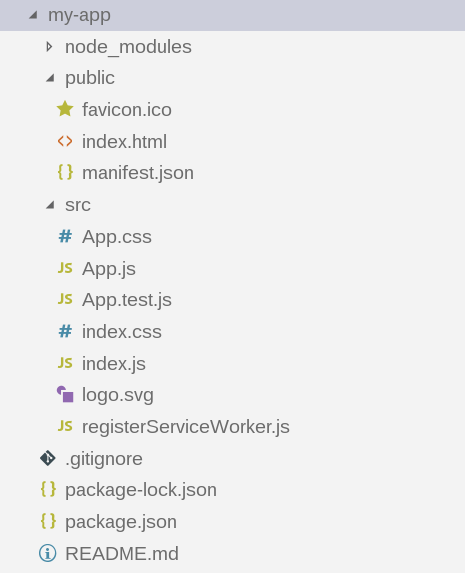
\includegraphics[width=\textwidth]{Ordnerstruktur}
          \caption{Die initiale Projektstruktur}
          \label{fig:init}
  \end{subfigure}
  ~ 
  \begin{subfigure}[t]{0.45\textwidth}
          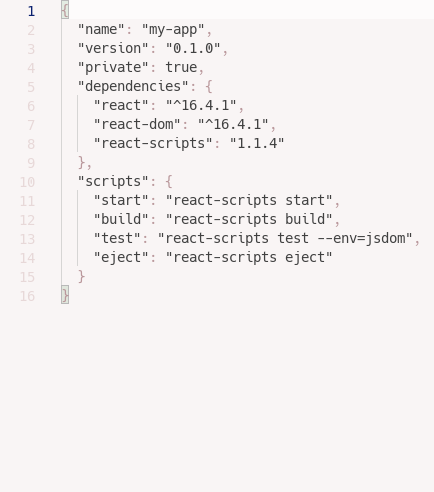
\includegraphics[width=\textwidth]{rca-package}
          \caption{Die initiale package.json Datei}
          \label{fig:init2}
  \end{subfigure}
  \grayRule
  \caption[Create React App: initiale Testapplikation]{einer mit Create React App erstellten Testapplikation}
  \label{fig:create-react-app}
\end{figure}

\subsub{Aufbau der React Komponenten}
\subsub{Online Offline}
React detect-offline
\subsub{lokale Datenbank}
Redux Offline: Idee: Store = Datenbank
\subsub{Backend}
CouchDB = RemoteDB\\
Redux Offline: Server der alle \gls{CRUD} Operationen unterstützt,
\gls{JSON}--Datei zur Persisierung um Ergebnisse nicht zu verfälschen 

%
%
% Architektur
%
\sub{Architektur}
\begin{figure}[H]
  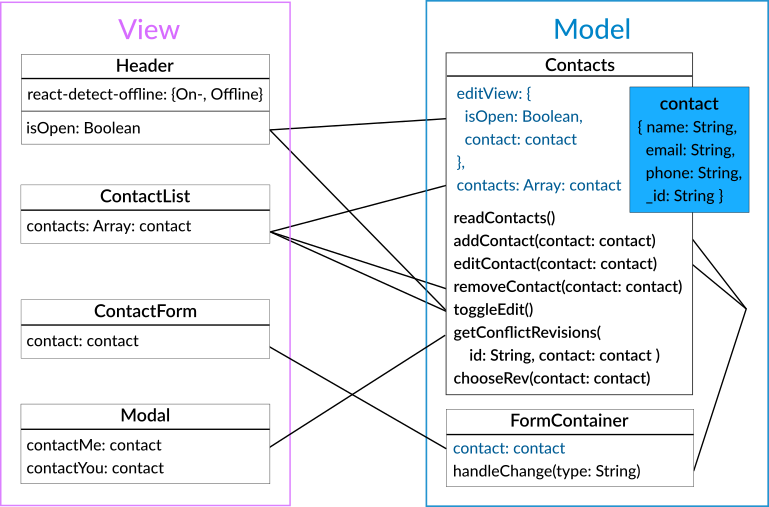
\includegraphics[width=\textwidth]{uml}
  \grayRule
  \caption{Komponentenarchitektur}
  \label{fig:uml}
\end{figure}

Container\\
Header\\
Liste\\
Form\\
Konflikt--Dialog\\
%
% Testfälle
%
\section{Testfälle}
Folgende Testfälle werden während der Entwicklung stetig durchgeführt. Das erfolgreiche Bestehen dieser Tests ist eine notwendige Qualitätseigenschaft / Voraussetzung der zu entwickelnden Prototypen.
\begin{itemize}
  	\item Netzwerkstatus anzeigen ? 
    \item Folgende Punkte müssten durch ServiceWorker usw sowohl on- als auch offline möglich sein. 
    \item Kontakt anlegen 
    \item Kontakt bearbeiten (Name, Email oder Telefonnummer)
    \item Kontakt löschen 
    \item lesen vorhandener Kontakte (lokal und Server)
\end{itemize}
%
% Entwicklungsumgebung
%
% \section{Entwicklungsumgebung}
% Für die Erstellung des Simulators wurde folgende Soft- und Hardware verwendet:
% \subsubsection{Software}
% \begin{itemize}
% 	\item Sublime Editor 3
% 	\item Visual Studio Code
% 	\item git, Version 2.7.4 zur Versionsverwaltung
% 	\item Inkscape, Version 0.92 zur Erstellung von Diagrammen und Zeichnungen
% \end{itemize}
% \subsubsection{Hardware}
% \begin{itemize}
% 	\item Tuxedo (Intel\textsuperscript{\textregistered} Core\tm i7-6500U, 2,50GHz x 4, 7,7 GB RAM) als ersten Entwicklungsrechner
% 	      (Betriebssystem: Ubuntu\footnote{ Download unter \url{https://www.ubuntu.com/download/desktop}} 16.06, 64-bit-Version)
% 	\item Lenovo Thinkpad X200 (Intel\textsuperscript{\textregistered} Core\tm   2 Duo, 2,40GHz, 8GB RAM) als zweiten Entwicklungsrechner (Betriebssystem: Debian 7.8, 64-bit-Version)
% \end{itemize}7